\chapter{Referencial Teórico}
\label{ref}
\section{Software Analytics}
\label{ref:sof}
Durante muito tempo a disponibilidade de dados em projetos de software para análise foi um problema. Hoje em dia, com o auxílio da internet, dos projetos de software livre e das características pervasivas e ubíquas da computação, o volume de dados a serem analisados se tornou um problema. Processar e analisar esses dados manualmente se tornou inviável\cite{artAndScience}. Atualmente, por exemplo, pesquisas mostraram que o \textit{Mozilla Firefox} teve 1.3 milhões de relatos de defeitos e outras plataformas como \textit{Sourcefoge.net} e o \textit{Github} hospedam 430.000 e 38 milhões de projetos, respectivamente\cite{informationNeeds}.

Na literatura não existe um consenso da definição de \textit{Software Analytics}, o livro~\cite{artAndScience} por exemplo,  define \textit{Software Analytics} como: "A análise de dados de software para gerentes e engenheiros de software, com o objetivo de capacitar indivíduos e times de desenvolvimento, a ganhar e difundir conhecimento a partir de seus dados para tomar melhores decisões". Essa atividade de análise ajuda a usuários, desenvolvedores e gerentes a responderem questões de introspecção, por exemplo, 'O por que e como um determinado evento ocorreu'. A utilização de \textit{Software Analytics} permite esse tipo de introspecção pois ao invés de propor e considerar a análise de métricas e dados independentemente, ela propõe diferentes tipos de análise em diferentes camadas de documentos, de forma a filtrar, resumir, modelar e realizar experimentações que permitam um melhor entendimento do que está acontecendo dentro do projeto\cite{informationNeeds}.

Hoje é comum empresas como Google, Facebook e Microsoft aplicarem métodos de análise de dados diariamente em seus projetos e produtos. Além disso, o número de conferências interessadas nos assuntos de mineração e análise de artefatos de software cresceu, destacando-se duas, a\textit{Mining Software Repositories} (MSR) e a \textit{PROMISE Conference on Repeatable Experimentes in Software Engineering}. Cada uma possui um foco diferente, sendo a MSR preocupada com a coleta dos dados, enquanto que a PROMISE com a eficácia e repetibilidade da análise de dados.

\subsection{Projetos \textit{Open Source} e Software Analytics}

A análise de dados obtidos de ferramentas de versionamento de código, como o Git, Bazaar, Subversion ou CVS pode trazer informações importantes a respeito da evolução de um projeto de software, por exemplo: o nível de engajamento dos desenvolvedores; o número de defeitos; a qualidade interna do produto; resultados de execução de testes, entre outros\cite{artAndScience}. O Github, uma das ferramentas mais utilizadas de versionamento de código-fonte atualmente, fornece uma API que permite a extração de dois tipos de dados:

\begin{itemize}
    \item \textbf{Metadados:} Os metadados fornecidos são informações associadas a cada \textit{commit} ou \textit{issue}, são: criador(a), data, mensagem do \textit{commit} ou \textit{issue}, a \textit{branch}, o repositório, e o escopo do \textit{commit} ou \textit{issue}. Além disso, na mensagem do \textit{commit} podem haver referencias a outros desenvolvedores, defeitos ou outros \textit{commits} e \textit{issues}.
    \item \textbf{Snapshots:} O código fonte do projeto, que pode ser obtido em diferentes fases do desenvolvimento, já que a ferramente permite que um usuário avance ou retroceda dentro dos \textit{commits}. Desta forma, é possível analisar o código de um projeto referente em vários períodos diferentes.
\end{itemize}

Abaixo, na figura~\ref{fig:github_api}, podemos ver o digrama de classes da API fornecida pelo Github, com base nesta imagem, é possível ver que as \textit{issues} e informações dos \textit{commiters} são exportadas a partir de um ponto comum de acesso.

\newpage
\begin{figure}[!h]
    \centering
        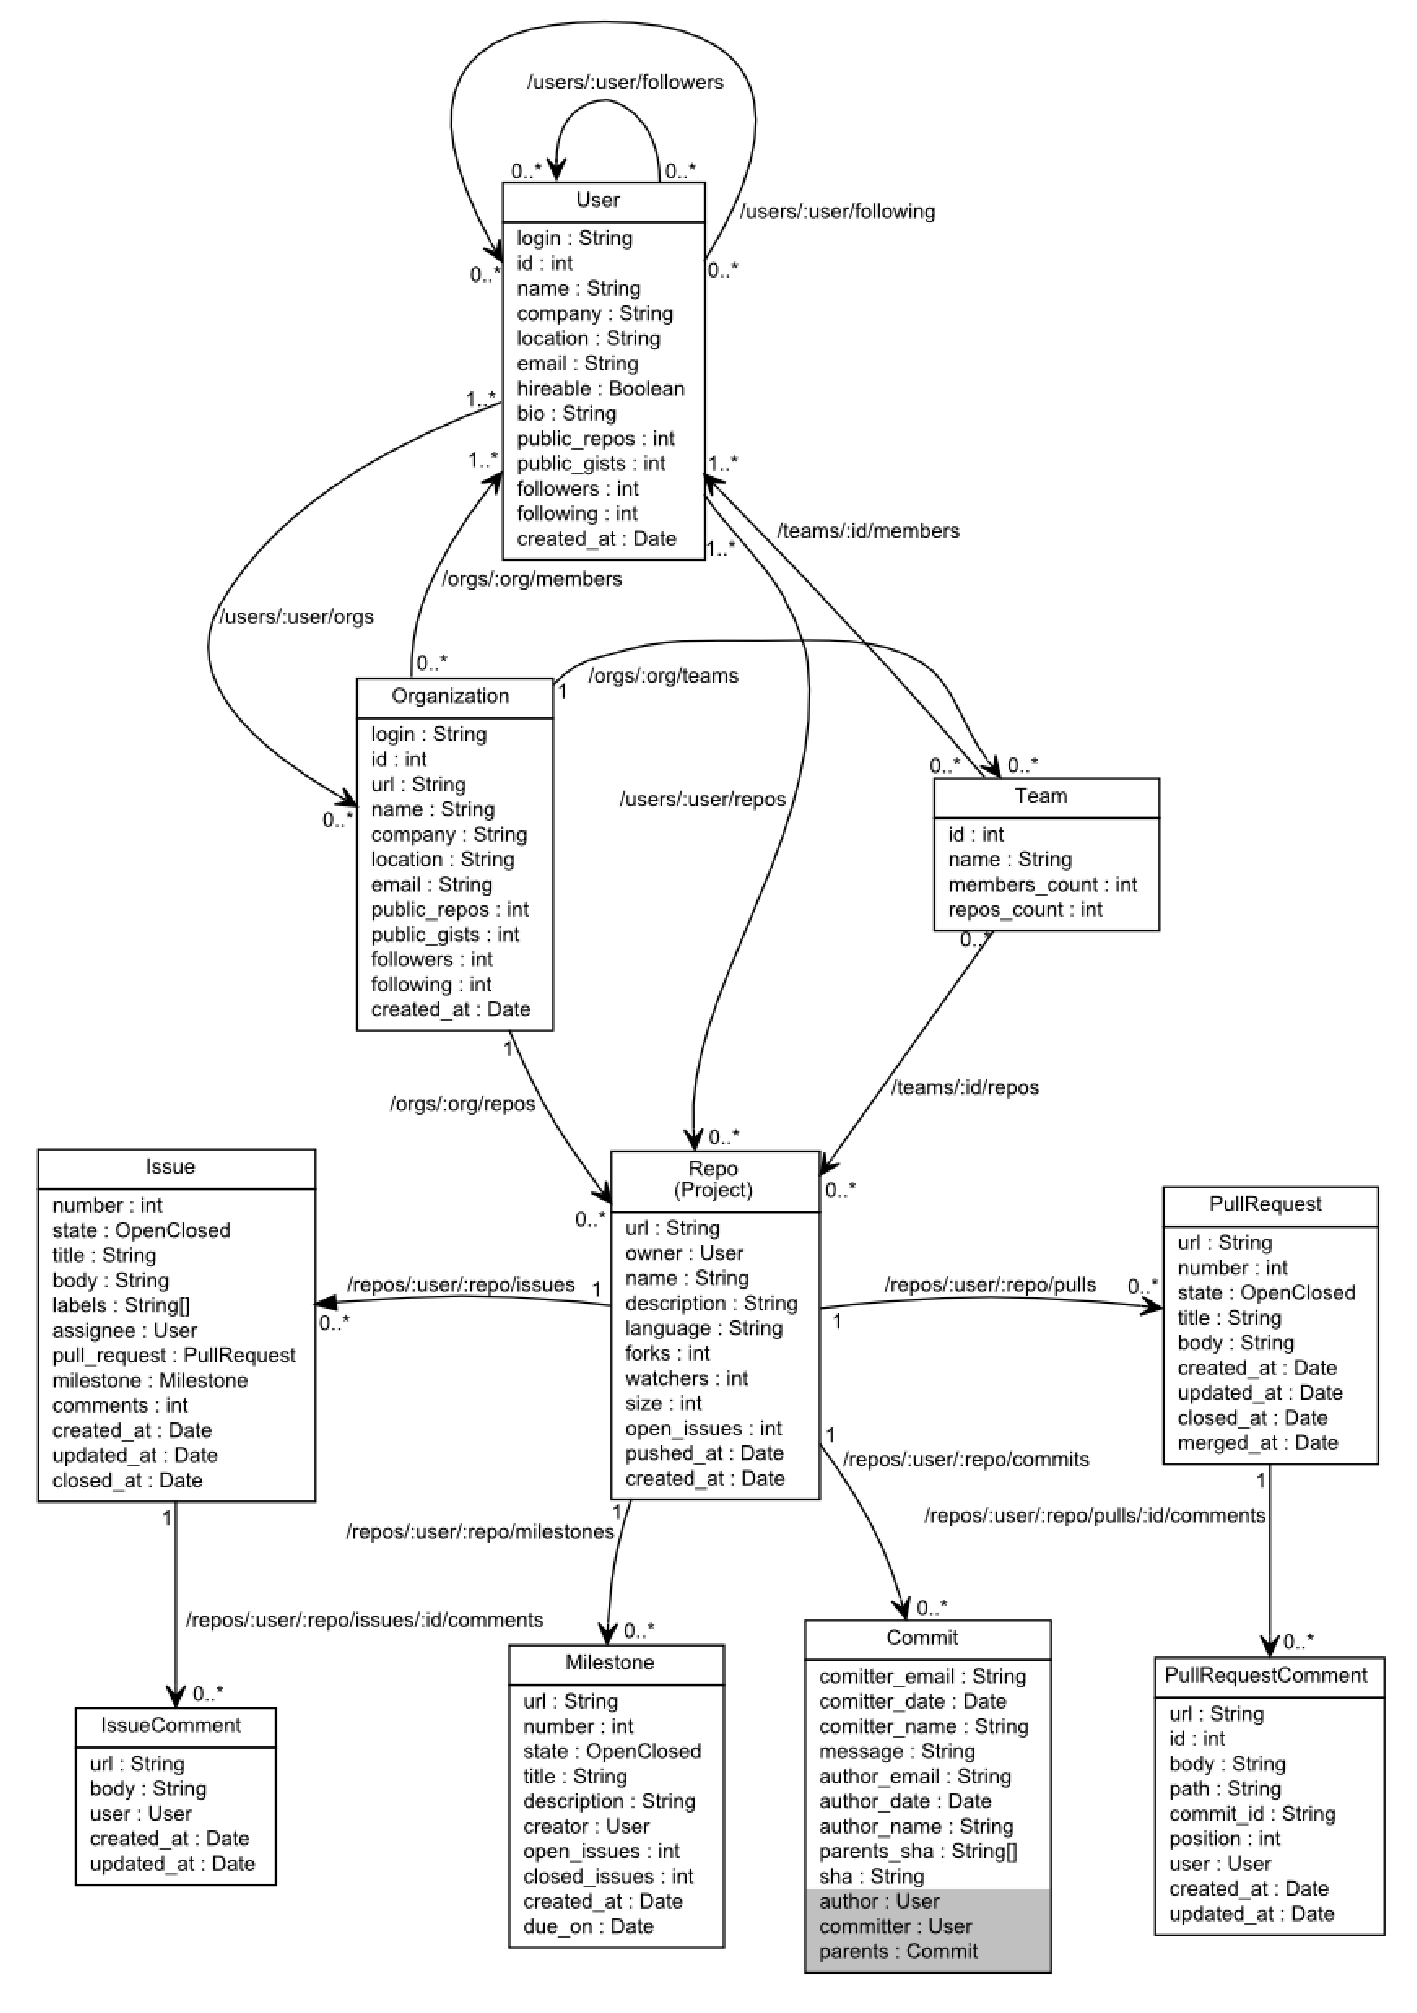
\includegraphics[width=\textwidth,height=\textheight,keepaspectratio=true]{figuras/gtschema.eps}
    \caption{Diagrama do Esquema do Github}
    \label{fig:github_api}
\end{figure}

\section{Desenvolvimento Ágil em Projetos \textit{Open Source}}
\label{red:des}

\subsection{Scrum}
O Scrum é um framework para o desenvolvimento e manutenção de produtos usado desde o incio dos anos 90 que possui a característica de permitir que vários processos e tecnicas possam ser empregadas juntamente a ele. Os três valores essenciais do Scrum são:

\begin{itemize}
    \item Leveza.
    \item Simples de entender.
    \item Difícil de dominar.
\end{itemize}

O Scrum é fundamentado nas teorias empíricas de controle de processo, ou seja, utiliza o conhecimento vindo de experiencias e das decisões passadas. Por isto, este  framework emprega uma abordagem iterativa e incremental para permitir aperfeiçoar a previsibilidade e os riscos. No Scrum, cada componente é essencial para o sucesso, por isso existem regras especificas para os times, artefatos e papéis dentro do framework.

\subsubsection{Práticas do Scrum}
\label{est:sof:met:pra}

O Scrum define algumas práticas que são aplicadas durante o desenvolvimento com o objetivo de minimizar a necessidade de reuniões. Estas práticas podem ser eventos com uma duração definida e buscam aumentar as interações entre as pessoas. A lista abaixo apresenta esses eventos e suas respectivas descrições.

\begin{itemize}
    \item \textbf{Sprint:} Um intervalo de tempo em que são desenvolvidos os itens
        propostos. Este intervalo geralmente é de duas a quatro semanas e ao final
        de cada sprint, um incremento de software é entregue.
    \item \textbf{Sprint Review:} Ao final de cada sprint o time revisa as atividades
        realizadas durante o período em que a sprint ocorreu. São levantados pontos de
        melhoria e quais foram os pontos fortes do time.
    \item \textbf{Sprint Planning:} No inicio de cada sprint, é feita uma reunião em
        que são priorizadas as atividades que serão realizadas.
    \item \textbf{Product Backlog:} Conjunto de itens que serão desenvolvidos no projeto.
        A cada sprint um conjunto de itens são escolhidos, retirados do \textit{Product
        Backlog} e implementados.
\end{itemize}

\subsection{Extremme Programming}




\subsection{Repositórios de Software e Metodologias Ágeis}




\section{Ranqueamento de Páginas e Centralidade de Redes}
\label{ref:ran}

\subsection{Centralidade}
\label{ref:ran:cen}
Centralidade é um dos tópicos mais estudados na teoria dos grafos, sendo um tópico de grande importância em estudos de redes sociais. Ela determina o grau de importância de um vértice dentre todos os outros dentro de uma rede. Na figura \ref{fig:centrality} é ilustrado um exemplo de centralidade. O conceito de centralidade de redes já foi aplicado a diversos contextos, dentre eles: investigar a influencia de redes inter organizacionais, estudos de relevância, vantagens em redes de troca, competência em organizações formais, oportunidades de emprego e diversos outros campos do mercado e ciência\cite{centrality}.

\begin{figure}[!h]
    \centering
        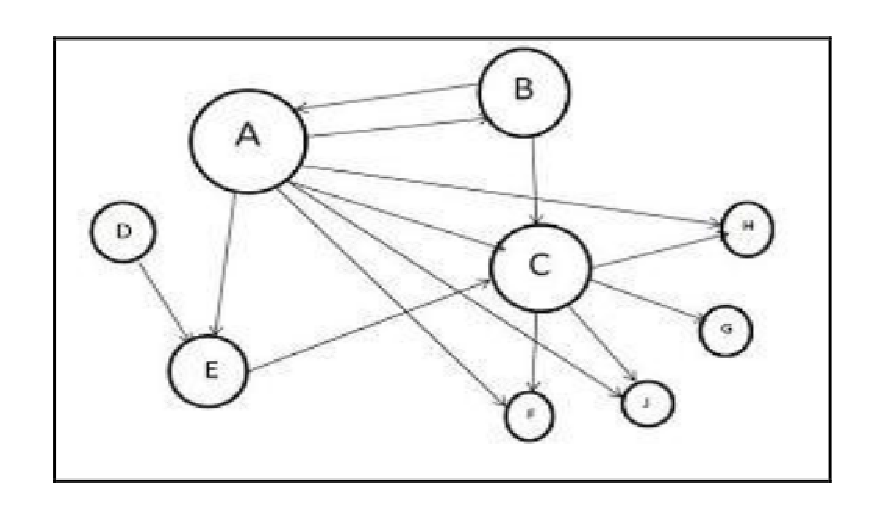
\includegraphics[keepaspectratio=true,scale=0.5]{figuras/centrality.eps}
    \caption{Exemplo de Relevância de um Nó em uma Rede}
    \label{fig:centrality}
\end{figure}

Diversos processos comumente encontrados no dia-a-dia são caracterizados por um fluxo. Esses processos diferem em dimensão e tipo, mas ainda assim podem ser comparados e exemplificados. Considerando que os processos de XXXX representam um fluxo, então podemos descrevê-los sob a perspectiva da Teoria dos Grafos\cite{ceflow}. Por exemplo:

\begin{itemize}
\item Dinheiro: Considere uma moeda, ou nota de um dólar, que se move pela economia e muda de mãos a cada transação. Uma nota é indivisível e só pode estar em um lugar em um determinado período de tempo. Na perspectiva da teoria dos grafos, a movimentação de uma nota em uma rede pode ser feita como um \textit{passeio (Walk)}, sendo, desta forma, representado como um processo de Markov.
\item Fofoca: Imagine uma informação privada que passa por uma rede de empregados de uma empresa. Diferentemente de uma moeda, essa mesma informação pode estar em diversos locais diferentes em um determinado período de tempo, se replicando a cada pessoa que passa a ter acesso a informação, mas geralmente não atravessa o mesmo vértice mais de uma vez, apesar de poder visitar o mesmo nó mais de uma vez. A movimentação desta informação em grafo pode ser representada como uma trilha\footnote{Em um grafo, uma trilha(\textit{trail}) é um passeio (\textit{Walk}) que não possui arestas repetidas}.
\item E-mail: Um vírus, ou spam de e-mail, que envia mensagens a todos os contatos de uma pessoa simultaneamente pode ser considerado um processo de fluxo. Um e-mail pode ser representado como uma trilha da mesma forma que é realizado com uma informação, já que compartilha propriedades semelhantes, como existir em diversos locais ao mesmo tempo, e geralmente, os e-mails não passam pelo mesmo vértice, ou caminho, duas vezes.
\item Infecções: O caso de uma infecção em que o hospedeiro ficou imune.
A infecção vão passar por duplicação de pessoa a pessoa, mas nunca vai voltar a infectar aqueles que já se tornaram imunes.
\item Pacotes: Um pacote de rede tem a característica de possuir um remetente e um destinatário. Normalmente é preferível que o pacote percorra o menor caminho possível até chegar ao seu destino. Dessa forma, a movimentação do pacote deve seguir o caminho geodésico\footnote{Um caminho geodésico em um grafo é composto pelas arestas que representam o menor caminho entre dois vértices.} pela rede de roteadores. 
\end{itemize}

\todo[inline, backgroundcolor=yellow!20!white, bordercolor=red]{Aqui faltou um parágrafo para alinhar a idéia desses exemplos com o foco que você pretende dar no seu caso em particular da investigação sobre centralidade.}

Ao longo dos anos, diferentes métodos de medida de centralidade foram criados, entre eles: Centralidade de Grau, Proximidade \textit{(Closeness)}, Intermediação \textit{(Betweenness)}, Autovetor \textit{(Eigen Vector)}, Informação, Intermediação de Fluxo, \textit{Rush Index}, Medidas de Influencia de Katz, Hubbell, Hoede e Taylor. Estes métodos diferem nas suposições iniciais que fazem para alcançar o objetivo de determinar o nó com maior importância, por exemplo, o algoritmo de Freeman de proximidade e intermediação conta apenas os caminhos geodésicos entre os nós, assumindo que qualquer fluxo que percorra uma rede, siga sempre pelo caminho mais curto.Outros algoritmos como a centralidade de autovetor de Bonacich conta travessias, o que assume que as trajetórias podem ser sinuosas, atravessando nós e arestas repetidas vezes até chegar ao destino\cite{centrality}.

\subsection{Ranqueamento de Páginas}
\label{ref:ran:pag}
O algoritmo de ranqueamento de páginas foi criado por Larry Page e Sergey em 1996. Ele permite calcular a importância relativa de páginas da web e tem aplicações em mecanismos de busca, estimativas de trafego e navegação na web. O algoritmo foi criado com o intuito de prover uma solução de busca de informações na web a partir da estrutura dos links, usada no hipertexto da web. \cite{pageRank}.

A premissa do algoritmo de ranqueamento de páginas é que cada página na web possui um número de links de saída e de entrada, e que páginas com um grande número de links são mais importantes do que as com poucos links. Além disso, o algoritmo também leva em consideração a relevância dos links de entrada de uma página, ou seja, se uma página da web possui um link de entrada que possui uma alta relevância, essa página tende a ser mais importante que outra que possua vários links mas que vieram de lugares mais obscuros \textcolor{red}{o que é mais obscuros?}.

A função de ranqueamento de páginas é definida na seguinte forma:

Seja $x$ uma página da web. Então
\begin{itemize}
    \item $L(x)$ é o conjunto de websites que possuem link para $x$
    \item $C(y)$ é o grau de entrada de $y$
    \item $\alpha$ é a probabilidade de um pulo aleatório
    \item $N$ é o número total de websites
\end{itemize}
\[\displaystyle PR(x) := \alpha \left ( \frac{1}{N} \right ) + (1-\alpha) \sum_{y\in L(x)} \frac{PR(y)}{C(y)}\]

Aplicando a equação acima, é possível obter o ranque de uma página, dado um conjunto de web-sites avaliados. \textcolor{red}{Explique melhor a função/aplicação.}

 Na figura \ref{fig:page_rank} é apresentado um exemplo como a relevância de uma página influencia as páginas seguintes.

\begin{figure}[!h]
    \centering
        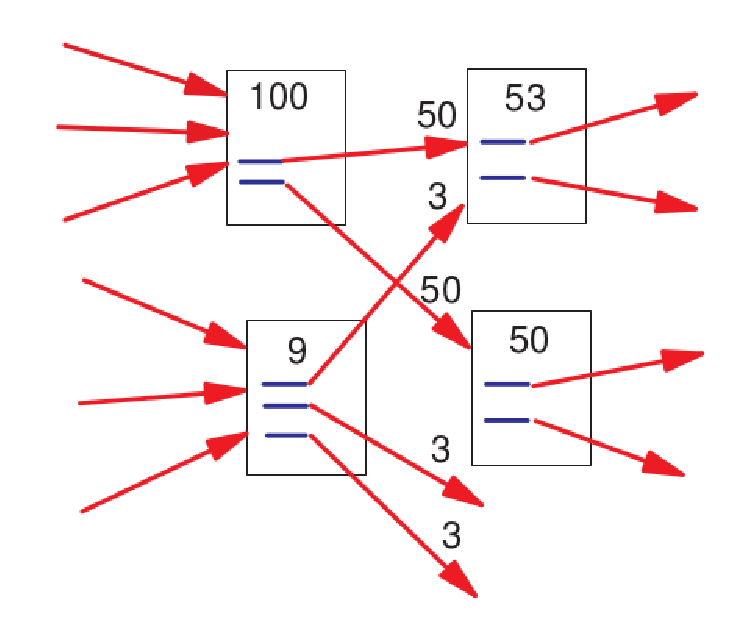
\includegraphics[keepaspectratio=true,scale=0.5]{figuras/page_rank.eps}
    \caption{Simplificação do Cálculo de Ranqueamento de Páginas}
    \label{fig:page_rank}
\end{figure}

\begin{figure}[!h]
    \centering
        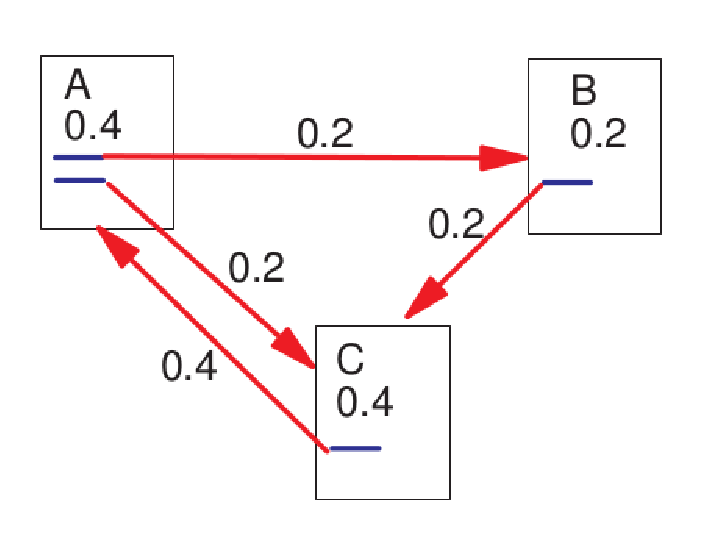
\includegraphics[keepaspectratio=true,scale=0.5]{figuras/page_rank2.eps}
    \caption{Simplificação do Cálculo de Ranqueamento de Páginas}
    \label{fig:page_rank2}
\end{figure}

Na figura \ref{fig:page_rank} é ilustrado como o ranqueamento de páginas se divide através das paginas e como ele contribui para o ranque das páginas seguintes. Já na figura \ref{fig:page_rank2} é ilustrado como um estado estável pode ser alcançado depois que o algoritmo é executado em um conjunto de páginas. 

\begin{figure}[!h]
    \centering
        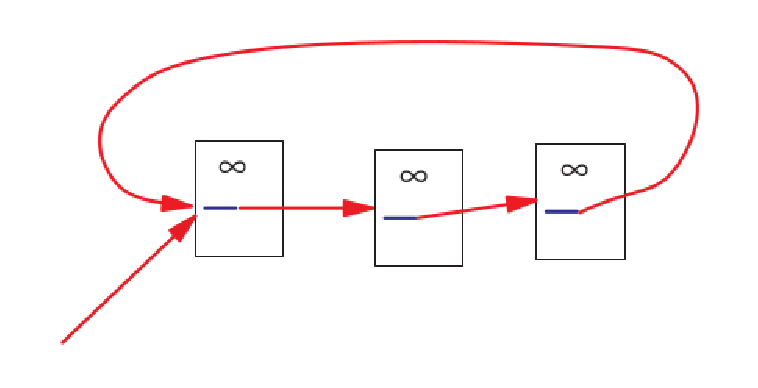
\includegraphics[keepaspectratio=true,scale=0.5]{figuras/page_rank3.eps}
    \caption{\textit{Loop} de Ranqueamento}
    \label{fig:page_rank3}
\end{figure}

Um dos problemas dessa função de ranqueamento, é que caso duas páginas da web que apontem uma para outra, e uma terceira aponte para qualquer uma destas, o \textit{loop} vai acumular ranque porém, nunca vai distribuir isso para nenhuma outra página seguinte. Na ilustração apresentada na figura~\ref{fig:page_rank3}, possível observar esse fenômeno.
